% ----------------------------------------------------------------
% Section: Background
% ----------------------------------------------------------------
\chapter{BACKGROUND}
\label{ch:background}

This section deals with survey of the key technologies and concepts underpinning the project.

\section{Android Automotive OS}
\label{sec:bg_aaos}

Android Automotive OS (AAOS) is a full-stack in-vehicle operating system derived from AOSP. Unlike Android Auto --- which mirrors a phone onto a head unit --- AAOS runs directly on the vehicle's IVI hardware \cite{aaos_overview}. It exposes automotive-specific APIs (vehicle properties, HVAC, driving state restrictions) while retaining the full Android framework, making it suitable for both OEM-integrated experiences and third-party application deployment.

AAOS uses the same build system and security primitives as standard AOSP: the \texttt{lunch} target, Soong/Make hybrid build rules, and the Android security model (SELinux, AVB, encryption). This project targets the \texttt{aosp\_rpi5\_car-bp4a} lunch target, producing a Bluetooth-primary Automotive variant.

Figure~\ref{fig:aaos_arch} shows the full AAOS system architecture across six layers. Security-relevant components are present at every layer --- from kernel-level SELinux and dm-verity, through HAL-level KeyMint and DRM, to framework and application-level permission and certificate management.

\begin{figure}[h]
\centering
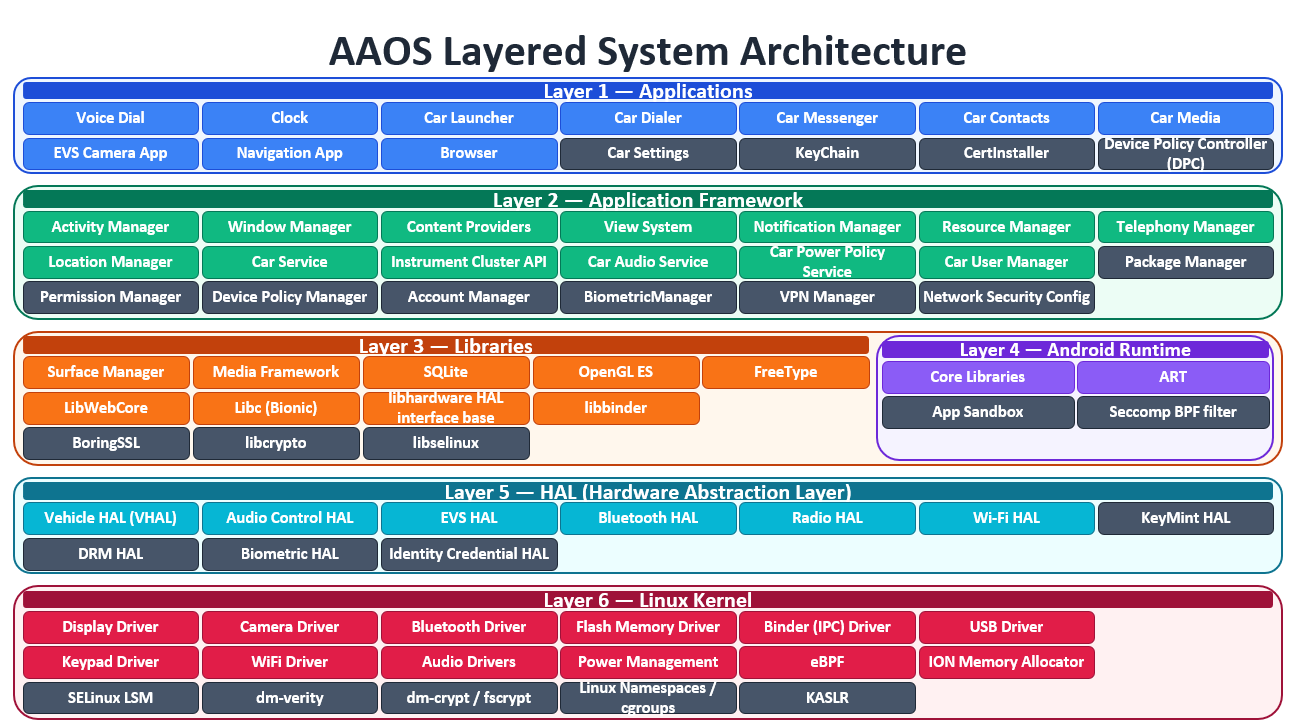
\includegraphics[width=\textwidth]{figures/aaos_system_architecture.png}
\caption{AAOS system architecture. Six layers from Linux Kernel (bottom) to Applications (top), with automotive-specific components (Vehicle HAL, Car Service, EVS) and security modules highlighted at each layer. Source: \cite{android_architecture_overview, android_security_features, aaos_overview}.}
\label{fig:aaos_arch}
\end{figure}

Not all security blocks in Figure~\ref{fig:aaos_arch} are within this project's scope.
Table~\ref{tab:arch_scope} identifies the subset that this project directly configures or
enables, distinguishing them from components that are either provided by base AOSP unchanged
or absent on the RPi~5 hardware (for example, no Biometric HAL or DRM Widevine is required
for a development automotive target).

\begin{table}[h]
\centering
\caption{Project-scope security blocks within the AAOS architecture}
\label{tab:arch_scope}
\begin{tabular}{llp{6.5cm}}
\toprule
\textbf{Layer} & \textbf{Block} & \textbf{Project action} \\
\midrule
Linux Kernel & SELinux LSM      & Enforcing mode enabled; policy validated at runtime \\
Linux Kernel & dm-verity        & AVB2 hashtree applied to \texttt{system} and \texttt{vendor} partitions \\
Linux Kernel & fscrypt          & File-Based Encryption activated on \texttt{/data} \\
HAL          & KeyMint HAL      & Used for AVB root-key storage and FBE key wrapping \\
HAL          & Vehicle HAL      & Required AAOS component; present via RPi5 device tree \\
\bottomrule
\end{tabular}
\end{table}

\section{Android Security Architecture}
\label{sec:bg_android_security}

Android implements a multi-layered security model in which hardware-backed trust mechanisms, OS-level isolation, and application-level controls reinforce one another \cite{android_security_features}. The key layers are:

\begin{description}
    \item[\textbf{Application Sandbox}]
    Each Android application is assigned a unique Unix UID and runs in its own isolated process. The Linux kernel enforces UID-based access controls, preventing one application from directly accessing another's data or code without explicit inter-process communication.

    \item[\textbf{Verified Boot (AVB)}]
    Establishes a hardware-rooted chain of trust from the bootloader through to all verified partitions using cryptographic signatures. Any modification to a verified partition is detected before the OS is allowed to start. (Detailed in Section~\ref{sec:bg_avb}.)

    \item[\textbf{SELinux}]
    Enforces Mandatory Access Control (MAC) over all processes and files, including those running with root or superuser privileges, constraining the damage any single compromise can cause.
    (Detailed in Section~\ref{sec:bg_selinux}.)

    \item[\textbf{Encryption}]
    Three complementary mechanisms protect data at rest: File-Based Encryption (FBE, Section~\ref{sec:bg_fbe}) encrypts each file independently with a per-file key; Full-Disk Encryption (FDE, Section~\ref{sec:bg_fde}) is the legacy block-level approach; and metadata encryption protects filesystem metadata (directory tree, file sizes, permissions) that FBE does not cover.

    \item[\textbf{Android Keystore}]
    Provides cryptographic operations (encryption, signing, key agreement) where the key material is stored inside a Trusted Execution Environment (TEE) or Secure Element, preventing key extraction even from a rooted device \cite{android_security_features}.

    \item[\textbf{Trusty TEE}]
    A minimal secure OS that executes on the same processor as Android but is isolated via hardware mechanisms (ARM TrustZone). It hosts security-sensitive services such as key storage, attestation, and biometric authentication.

    \item[\textbf{Gatekeeper and Weaver}]
    Gatekeeper performs PIN / pattern / password authentication inside the TEE and enforces hardware-backed lockout after repeated failures. Weaver provides an additional layer of credential binding in a dedicated secure element where available.

    \item[\textbf{App Signing}]
    All Android applications must be cryptographically signed before installation. Signing ties updates to a developer identity and underpins the package manager's integrity checks.
\end{description}

This project engages four of these layers directly: AVB (boot-time integrity), FBE (user-data encryption), SELinux (access control), and the Android Keystore (AVB key storage and FBE key wrapping).

\section{Raspberry Pi 5 Hardware}
\label{sec:bg_rpi5}

The Raspberry Pi~5 is built around the Broadcom BCM2712 SoC featuring:

\begin{itemize}
    \item Quad-core ARM Cortex-A76 at up to 2.4~GHz (64-bit AArch64)
    \item Up to 16~GB LPDDR4X RAM
    \item PCIe 2.0 x1 (exposed via the FFC connector)
    \item Dual 4K HDMI, USB 3.0, Gigabit Ethernet
    \item 40-pin GPIO header with UART on GPIO~14 (TX) and GPIO~15 (RX) \cite{rpi_uart_pinout}
    \item A dedicated 3-pin debug serial connector (between the HDMI ports)
\end{itemize}

The RPi5 firmware (VideoCore firmware) performs early hardware initialisation and hands off to the configured bootloader by reading \texttt{config.txt} from the FAT32 boot partition. By default it boots the Linux kernel Image directly, but it can be redirected to load \texttt{u-boot.bin} instead \cite{rpi_hardware_docs}.

One key difference from earlier RPi boards is that the primary UART (\texttt{serial10}) is exposed via an AXI-connected PL011 UART instance, declared in the firmware Device Tree as \texttt{compatible = "arm,pl011-axi"} rather than the standard \texttt{"arm,pl011"} string \cite{arm_pl011_trm}.

\section{U-Boot Bootloader}
\label{sec:bg_uboot}

U-Boot is a widely-used open-source bootloader for embedded systems. It provides a scriptable boot environment supporting multiple storage media (MMC, NVMe, USB, network TFTP) and is cross-compiled for AArch64 using \cite{uboot_build_gcc}:

\begin{lstlisting}[language=bash]
CROSS_COMPILE=aarch64-linux-gnu- make rpi_arm64_defconfig
CROSS_COMPILE=aarch64-linux-gnu- make -j$(nproc)
\end{lstlisting}

U-Boot uses a Driver Model (DM) architecture where peripheral drivers declare compatible strings in a \texttt{udevice\_id} table \cite{uboot_serial_pl01x}. The boot sequence is controlled by a compiled script (\texttt{boot.scr}) produced by \texttt{mkimage}. Initial RPi5 support landed in U-Boot v2024.04; however, several limitations remained, particularly around PCIe, USB, and Ethernet initialisation \cite{uboot_rpi5_forum, rpi5_uboot_boot_issues}.

\subsection{U-Boot AVB Integration}

U-Boot's AVB support (\texttt{CONFIG\_AVB\_VERIFY}, \texttt{CONFIG\_CMD\_AVB}, \texttt{CONFIG\_LIBAVB}) allows it to invoke the \texttt{avb verify} command to check partition signatures before booting. The public key used for verification is compiled directly into \texttt{common/avb\_verify.c} as a C array (\texttt{avb\_root\_pub[]}).

\section{Android Verified Boot 2.0 (AVB)}
\label{sec:bg_avb}

Android Verified Boot 2.0 (AVB2) is Google's cryptographic boot-time integrity framework, defined as ``the process of assuring the end user of the integrity of the software running on a device'' \cite{avb2_readme}. The central data structure is the \emph{VBMeta image}:a signed metadata partition whose descriptors span all verified partitions, establishing a \emph{chain of trust} rooted in the public key compiled into the bootloader.

\subsection{VBMeta Descriptors}
\label{sec:bg_avb_descriptors}

The VBMeta structure is cryptographically signed (SHA-256 / RSA-4096) and contains one or more typed descriptors \cite{avb2_readme}:

\begin{description}
    \item[\textbf{Hash descriptor}]
    Records the SHA-256 hash of an entire partition image (ex:\ \texttt{boot}). Verification confirms the partition has not been modified since signing.

    \item[\textbf{Hashtree descriptor}]
    Used for large ext4 partitions (\texttt{system}, \texttt{vendor}). A 4~KiB-block Merkle tree (SHA-256) is appended to the partition image; the descriptor stores the root hash, salt value, and hashtree offset. At runtime, \texttt{dm-verity} enforces block-level integrity by recomputing hashes on each read \cite{android_dm_verity}.

    \item[\textbf{Kernel commandline descriptor}]
    Carries verified kernel parameters that are passed to the kernel by the bootloader after successful verification. This allows security-relevant cmdline flags (ex:\ \texttt{androidboot.verifiedbootstate}) to be integrity-protected.

    \item[\textbf{Chained partition descriptor}]
    Delegates verification authority to a separate VBMeta image residing on another partition, together with the trusted public key for that image. This enables independently signed partitions to participate in the chain of trust without embedding their hashes directly in the top-level VBMeta.
\end{description}

Figure~\ref{fig:avb_basic} illustrates a typical AVB configuration where the top-level VBMeta partition holds hash and hashtree descriptors for \texttt{boot},
\texttt{system}, and \texttt{vendor}.

\begin{figure}[h]
\centering
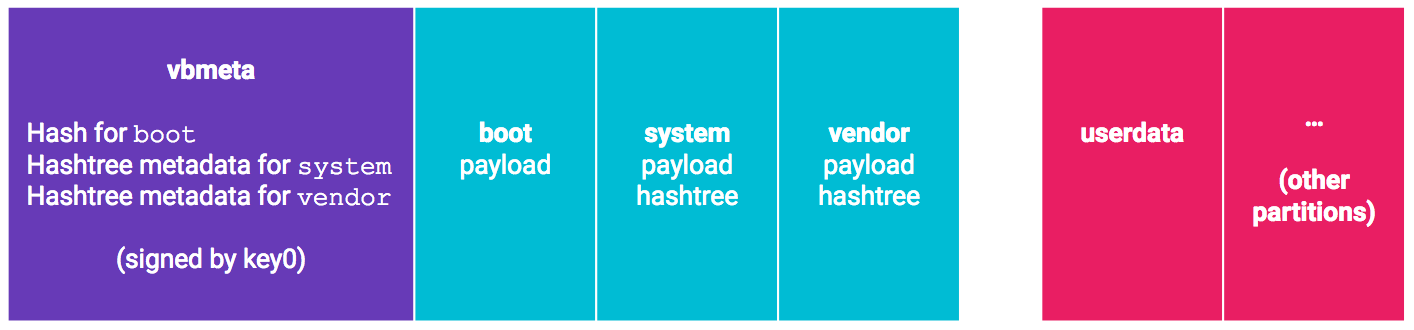
\includegraphics[width=\textwidth]{figures/avb_basic_partitions.png}
\caption{AVB with \texttt{boot}, \texttt{system}, and \texttt{vendor} partitions. The \texttt{vbmeta} partition holds signed descriptors for all three. Source: \cite{avb2_readme}.}
\label{fig:avb_basic}
\end{figure}

Figure~\ref{fig:avb_chained} shows chained partition delegation, where the top-level VBMeta delegates authority to a per-partition VBMeta image via a public key embedded in the chained descriptor.

\begin{figure}[h]
\centering
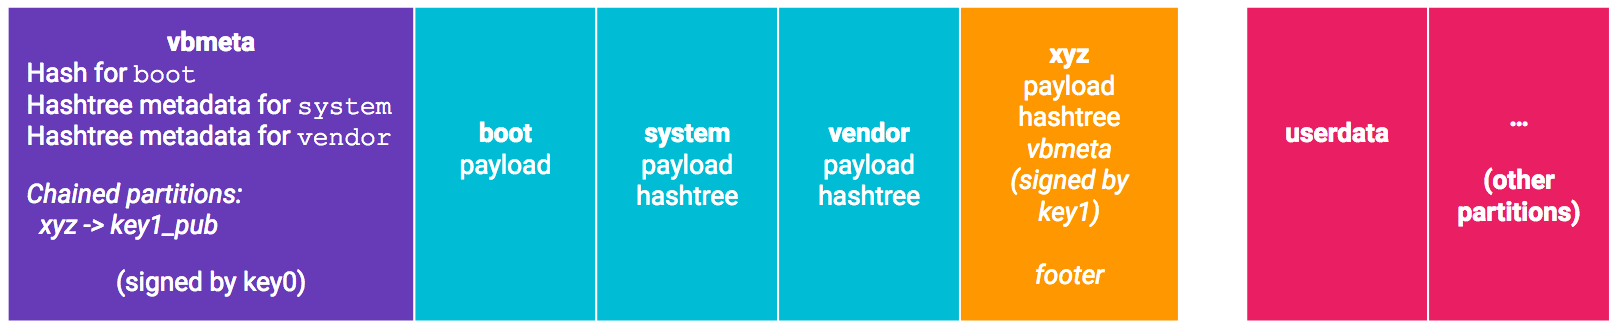
\includegraphics[width=\textwidth]{figures/avb_chained_partition.png}
\caption{AVB with a chained partition: the top-level \texttt{vbmeta} embeds the public key used to verify an independently signed partition's own VBMeta image. Source: \cite{avb2_readme}.}
\label{fig:avb_chained}
\end{figure}

\subsection{Rollback Protection}
\label{sec:bg_avb_rollback}

AVB maintains \emph{rollback indices}: monotonically increasing integers stored in tamper-evident persistent storage on the device. Each signed image carries a minimum required rollback index value; the bootloader rejects any image whose rollback index is below the stored value, preventing downgrade attacks that would re-expose patched vulnerabilities \cite{avb2_readme}.

Figures~\ref{fig:avb_rollback} and~\ref{fig:avb_stored_rollback} illustrate how rollback index values are embedded in partitions and compared against the values stored on the device.

\begin{figure}[h]
\centering
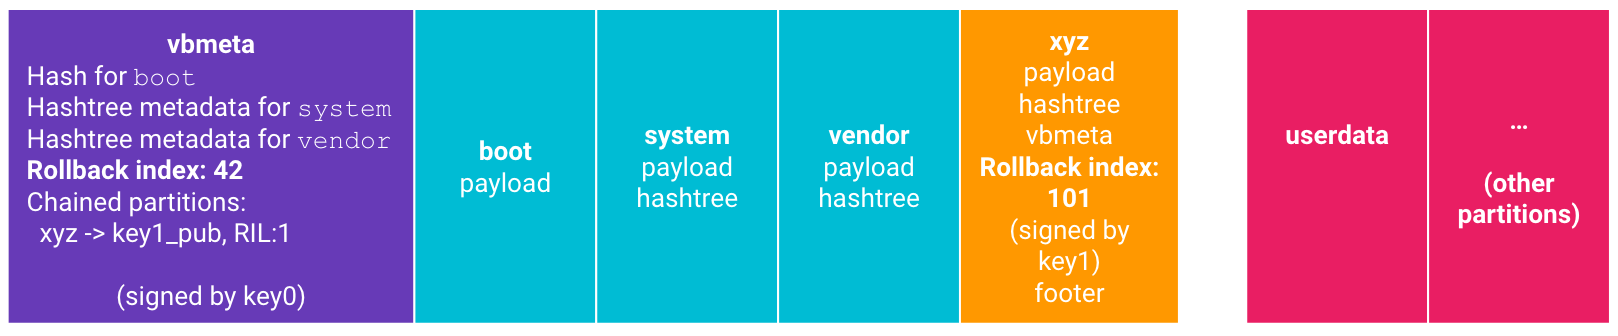
\includegraphics[width=0.85\textwidth]{figures/avb_rollback_indexes.png}
\caption{AVB rollback index values embedded in \texttt{vbmeta} and partition images. Source: \cite{avb2_readme}.}
\label{fig:avb_rollback}
\end{figure}

\begin{figure}[h]
\centering
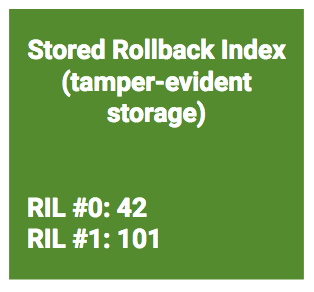
\includegraphics[width=0.6\textwidth]{figures/avb_stored_rollback_indexes.png}
\caption{Device-stored rollback index locations. Values must be $\geq$ those in the signed metadata for boot to proceed. Source: \cite{avb2_readme}.}
\label{fig:avb_stored_rollback}
\end{figure}

\subsection{Device States and Boot Colour Model}
\label{sec:bg_avb_states}

AVB defines two device modes and a four-colour boot state model \cite{avb2_readme}:

\begin{description}
    \item[\textbf{Locked mode}] Full verification is enforced. The bootloader verifies the VBMeta signature against its compiled-in root public key before loading any partition.

    \item[\textbf{Unlocked mode}] Verification may be bypassed (ex:\ for development), but the device advertises an \texttt{orange} boot state to the Android framework.
\end{description}

The four boot colour states reported via \texttt{androidboot.verifiedbootstate} are: \texttt{green} (full verification passed with OEM key), \texttt{yellow} (verification passed with a non-OEM key), \texttt{orange} (unlocked / bypass mode), and \texttt{red} (verification failed or image corrupted) \cite{avb2_readme}.

\subsection{A/B Slot Support}
\label{sec:bg_avb_ab}

AVB is designed to work with A/B partitioned devices, where two copies of each updatable partition are maintained (\texttt{\_a} and \texttt{\_b} slots). This enables seamless over-the-air updates: the update writes to the inactive slot, which is then verified and activated on the next boot, while the active slot continues to serve the running system. The slot selection metadata is maintained outside the signed VBMeta, allowing the bootloader to switch slots without re-signing \cite{avb2_readme}.

\begin{figure}[h]
\centering
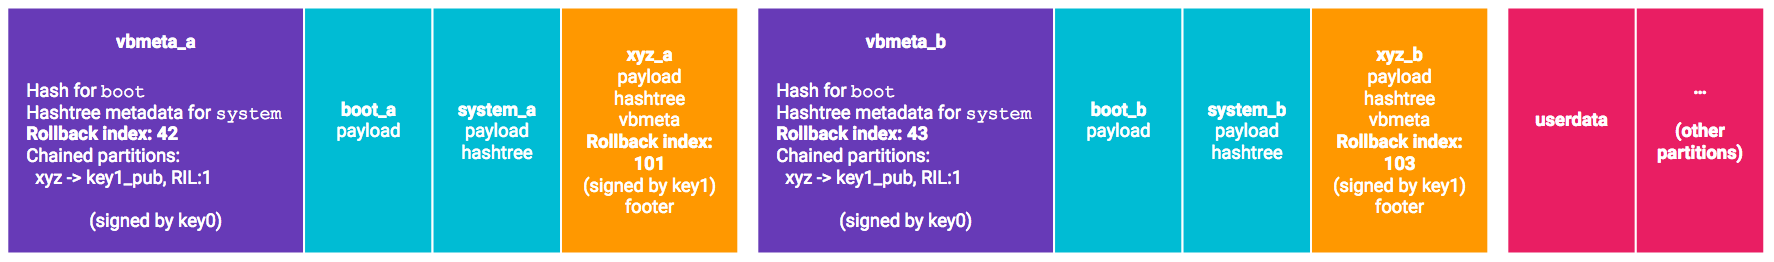
\includegraphics[width=\textwidth]{figures/avb_ab_partitions.png}
\caption{AVB with A/B partitions: both \texttt{\_a} and \texttt{\_b} slot images are independently signed; the bootloader selects and verifies the active slot. Source: \cite{avb2_readme}.}
\label{fig:avb_ab}
\end{figure}

\subsection{libavb and avbtool}
\label{sec:bg_avb_tools}

The \texttt{platform/external/avb} repository provides two key components
\cite{avb2_readme, avbtool_github}:

\begin{description}
    \item[\texttt{libavb}] A portable C library implementing the full AVB verification logic. It requires only a small set of I/O and crypto operations to be provided by the platform, making it suitable for integration into bootloaders such as U-Boot.

    \item[\texttt{avbtool}] A Python~3 command-line utility used at build time to generate hash and hashtree footers and to produce the final \texttt{vbmeta.img}. Key operations include \texttt{add\_hash\_footer}, \texttt{add\_hashtree\_footer}, and \texttt{make\_vbmeta\_image}.
\end{description}

The \emph{VBMeta digest} --- a cryptographic hash of the complete VBMeta partition contents --- is computed by \texttt{avbtool} and can be stored by the bootloader to detect any subsequent tampering of the VBMeta partition before the kernel is loaded \cite{avb2_readme}.

Figure~\ref{fig:avb_boot_flow} shows the recommended AVB boot flow, from bootloader initialisation through VBMeta verification to kernel handoff.

\begin{figure}[h]
\centering
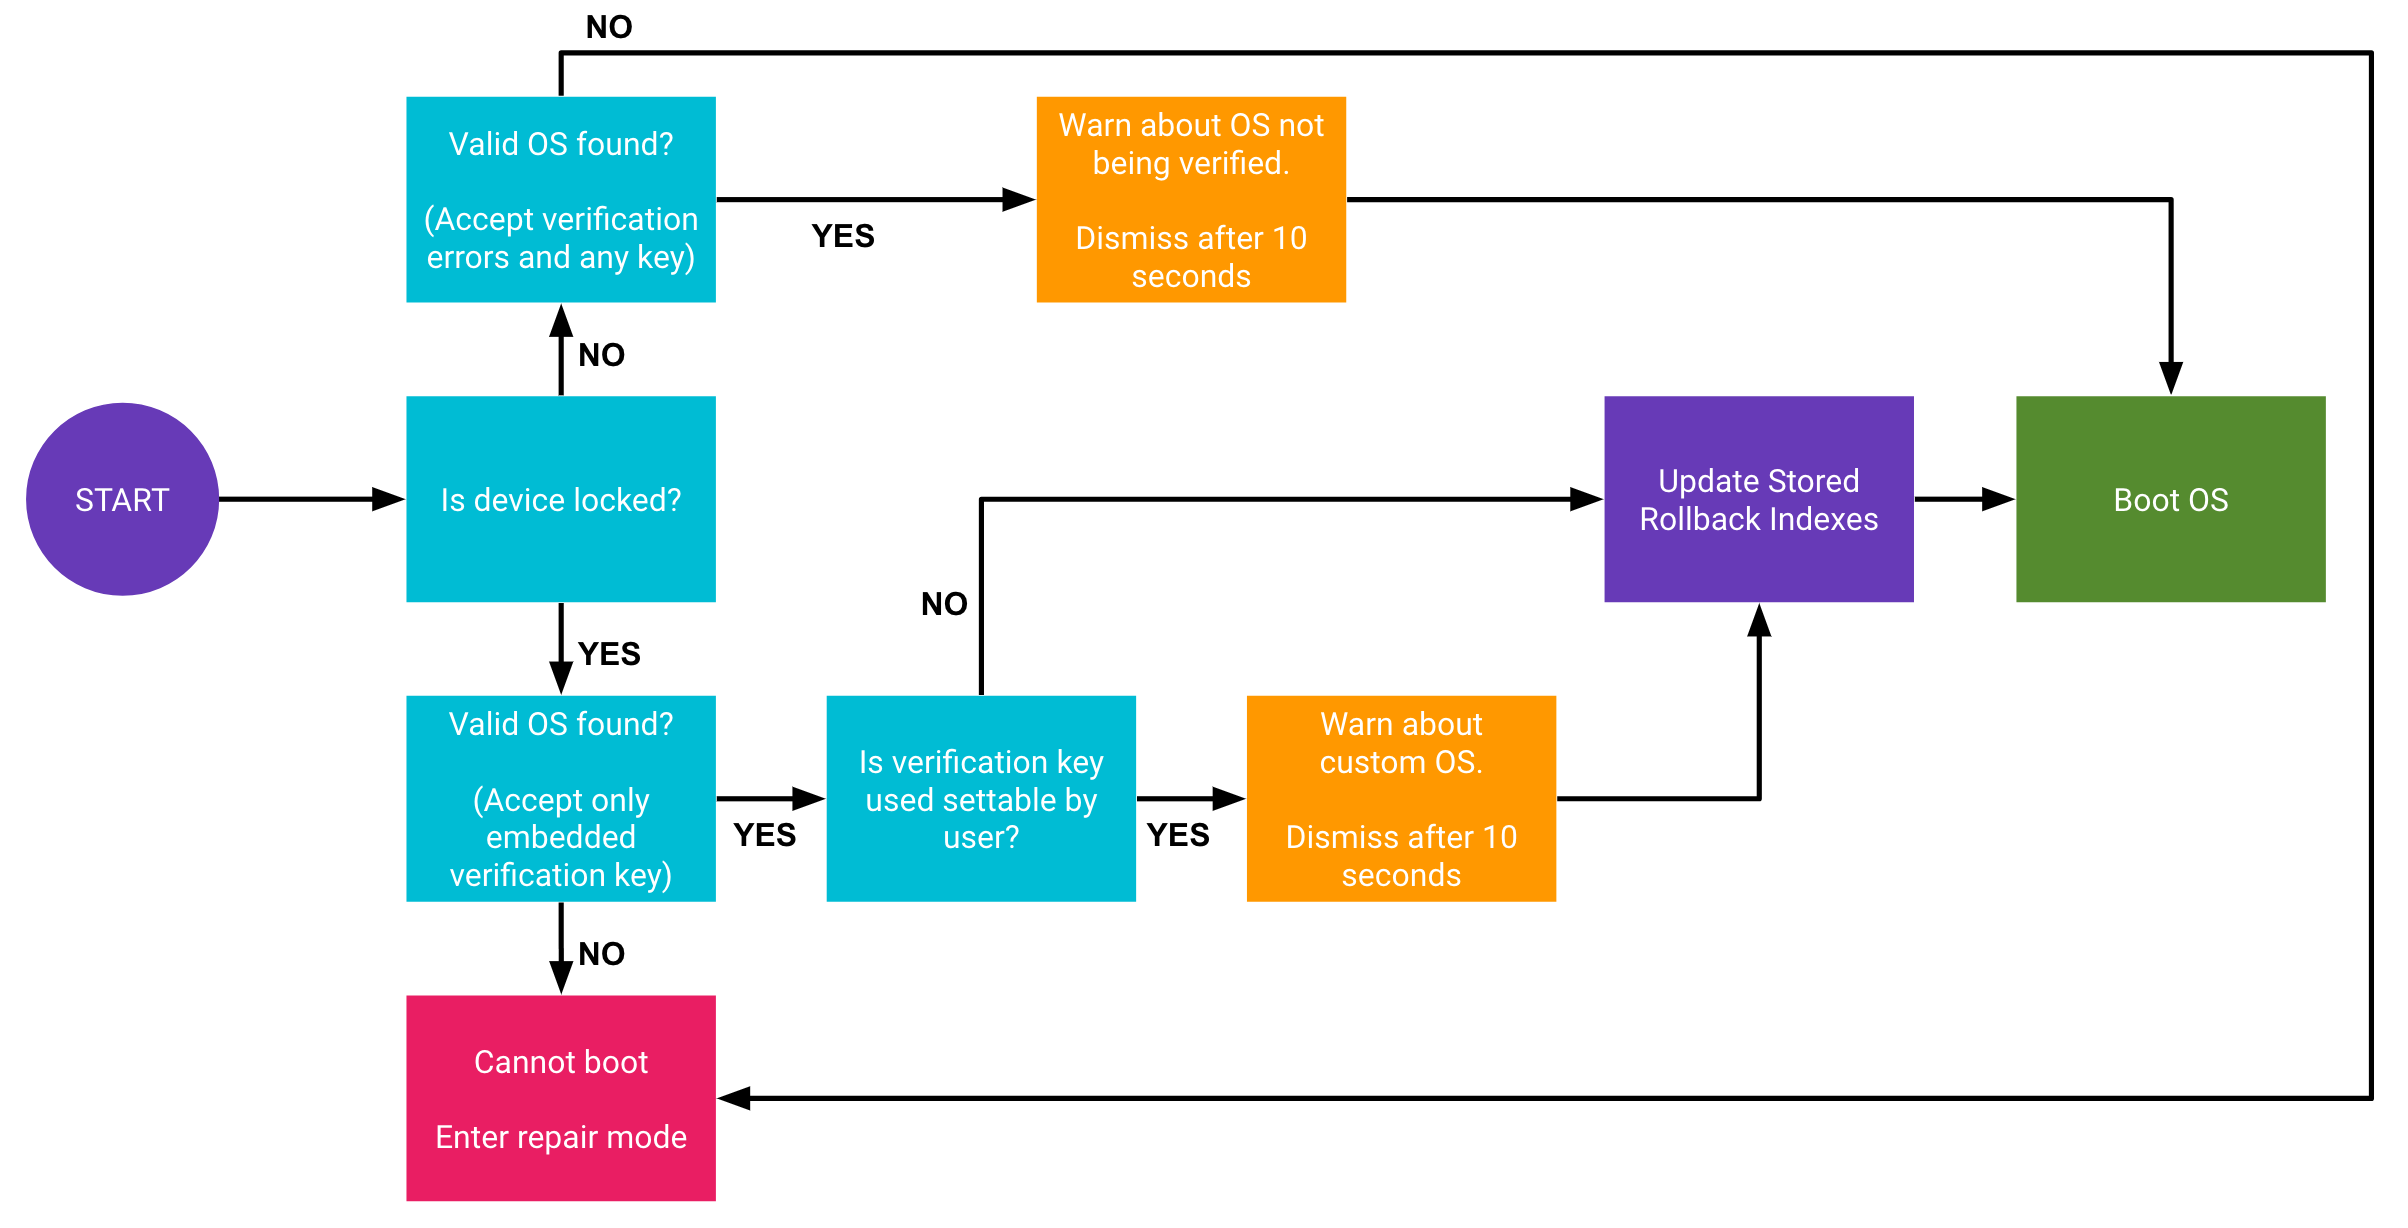
\includegraphics[width=0.75\textwidth]{figures/avb_boot_flow.png}
\caption{Recommended AVB boot flow: the bootloader verifies the VBMeta signature, checks rollback indices, validates partition hashes/hashtrees, and passes the verified boot state to the kernel via the commandline. Source: \cite{avb2_readme}.}
\label{fig:avb_boot_flow}
\end{figure}

\section{dm-verity}
\label{sec:bg_dmverity}

\texttt{dm-verity} is a Linux device-mapper target that enforces read-time block integrity using a Merkle hash tree \cite{android_dm_verity}. On Android, it is the runtime enforcement mechanism for the AVB hashtree. For every 4~KiB block read from a verified partition, the kernel computes its SHA-256 hash and compares it against the precomputed tree. Any mismatch triggers an I/O error or, in \texttt{restart\_on\_corruption} mode, reboots the device.

Android 7.0 and later enhanced \texttt{dm-verity} with forward error correction (FEC) using Reed-Solomon codes, reducing the likelihood of a single corrupt sector causing a boot failure.

\section{Full-Disk Encryption (FDE)}
\label{sec:bg_fde}

Full-Disk Encryption (FDE) is Android's legacy block-level encryption mechanism, introduced in Android 5.0 \cite{android_fde}. It encrypts the entire \texttt{/data} partition as a single block device using the Linux \texttt{dm-crypt} device-mapper target with 128-bit AES in CBC mode and ESSIV:SHA256. Devices launched on Android 10 or later are required to use FBE instead; FDE is completely removed in Android 13. Android 10--12 retain FDE support only for devices upgrading from Android 9 or earlier.

\subsection{Key Derivation Chain}
\label{sec:bg_fde_keys}

FDE protects the Disk Encryption Key (DEK) through a seven-step derivation chain that binds decryption to both the user's credential and a hardware key stored in the TEE \cite{android_fde}:

\begin{enumerate}
    \item Generate a random 16-byte DEK and a random 16-byte salt.
    \item Apply \texttt{scrypt} to the user password and the salt, producing a 32-byte intermediate key IK1.
    \item Pad IK1 with zeros to the size of the TEE-stored private key.
    \item Sign the padded value with the TEE hardware key, yielding IK2.
    \item Apply \texttt{scrypt} a second time to IK2 and the salt, producing a 32-byte IK3.
    \item Split IK3: the first 16 bytes become the Key Encryption Key (KEK); the last 16 bytes become the initialisation vector (IV).
    \item Encrypt the DEK using AES-CBC with KEK and IV, and store the result on the device.
\end{enumerate}

This chain ensures that recovering the DEK requires both the user's credential \emph{and} access to the TEE hardware key, preventing offline brute-force attacks on the encrypted partition.

\subsection{Boot Flow and Service Classes}
\label{sec:bg_fde_boot}

Because the entire \texttt{/data} partition is encrypted as a single unit, decryption must complete before any service that reads user data can start. Android manages this through three \texttt{init} service classes \cite{android_fde}:

\begin{description}
    \item[\texttt{core}] Services that must never stop, started immediately at boot.
    \item[\texttt{main}] Services that restart after the user provides their credential and decryption completes.
    \item[\texttt{late\_start}] Services that begin only after \texttt{/data} has been decrypted and remounted.
\end{description}

For default (no-password) encryption, \texttt{vold} detects the encrypted partition, creates a \texttt{dm-crypt} mapping using the stored DEK, and mounts the decrypted filesystem directly. For password-protected devices, a temporary \texttt{tmpfs} filesystem is mounted first to display the unlock UI; after credential verification, services in the \texttt{main} and \texttt{late\_start} classes are stopped, the real partition is decrypted and remounted, and those services restart. Coordination between \texttt{vold} and \texttt{init} uses properties: \texttt{vold.decrypt}, \texttt{vold.encrypt\_progress}, and \texttt{ro.crypto.state}.

\subsection{Limitations and Deprecation Rationale}
\label{sec:bg_fde_limitations}

FDE has two fundamental limitations that motivated its replacement by FBE
\cite{android_fde}:

\begin{enumerate}
    \item \textbf{No Direct Boot support.}  All files in \texttt{/data} share a single DEK. The OS cannot access \emph{any} user data --- including alarms, phone calls, or accessibility services --- until the user authenticates after reboot. FBE's per-file keys enable Device-Encrypted (DE) files to be available immediately.
    \item \textbf{Unrecoverable partial encryption.}  A power failure during the initial in-place encryption pass leaves \texttt{/data} in a partially encrypted state with no recovery path other than a factory reset.
\end{enumerate}

\section{File-Based Encryption (FBE)}
\label{sec:bg_fbe}

Android's File-Based Encryption (FBE), introduced in Android 7.0 and mandatory from Android 10, encrypts each file independently using the Linux \texttt{fscrypt} subsystem \cite{android_fbe}. It defines two encryption classes:

\begin{description}
    \item[Device Encrypted (DE)] Available immediately after boot, before user authentication. Used for files required during Direct Boot.
    \item[Credential Encrypted (CE)] Locked until the user provides credentials (PIN, password, or biometric).
\end{description}

Encryption is configured via \texttt{fstab} flags on the \texttt{userdata} partition: \path{fileencryption=aes-256-xts:aes-256-cts:v2}. A dedicated \texttt{/metadata} partition stores the key wrapping material managed by \texttt{vold} using the \texttt{keydirectory=} flag \cite{android_fbe, android_data_encryption}.

\section{SELinux on Android}
\label{sec:bg_selinux}

Android enforces Mandatory Access Control (MAC) through SELinux. From Android 8.0 onward, platform and vendor policies are built and versioned independently \cite{selinux_build_precompiled}. Device bring-up typically begins in \textit{permissive} mode (denials logged but not enforced), transitioning to \textit{enforcing} mode as policy matures \cite{selinux_device_policy}. Policy is precompiled at build time into \path{/vendor/etc/selinux/precompiled_sepolicy}; at boot, \texttt{init} validates it against SHA-256 hashes before loading.

\section{Android Init System}
\label{sec:bg_init}

Android's \texttt{init} is the first userspace process. It parses \texttt{.rc} files (Android Init Language) to manage services and trigger actions on property changes. First-stage init is responsible for mounting \texttt{/system} and \texttt{/vendor} from the \texttt{fstab}; at this point it also runs the AVB verification policy from the \texttt{fstab} \texttt{avb=} flags. Second-stage init handles service lifecycle, SELinux policy loading, and property management.

\section{ISO/SAE 21434 and Threat Analysis and Risk Assessment (TARA)}
\label{sec:bg_tara}

ISO/SAE 21434 \cite{iso_sae_21434} is the cybersecurity engineering standard for road vehicles. Its Threat Analysis and Risk Assessment (TARA) process (Clause~15) provides a structured methodology for identifying, evaluating, and treating cybersecurity risks in automotive systems. Although this project targets a research platform rather than a production automotive ECU, the TARA methodology is applied to characterise the security posture and to identify the gap between the current implementation and production-grade hardening requirements.

\subsection{Asset Identification}

An \emph{asset} is any component whose loss of confidentiality, integrity, or availability would harm the security posture or operational function of the system. Assets are categorised by type (credential, image, configuration, interface, build artifact, data) and annotated with the security properties at risk: Confidentiality~(C), Integrity~(I), and Availability~(A).

\subsection{STRIDE Threat Modelling}

Threats are enumerated by applying the STRIDE model \cite{stride_microsoft} to each asset:

\begin{description}
    \item[\textbf{S}poofing] An entity falsely claims to be another (ex:\ a fake AVB public key).
    \item[\textbf{T}ampering] Modification of data or code without authorisation (ex:\ altering a partition image on the SD card).
    \item[\textbf{R}epudiation] Denying that an action took place (ex:\ absence of a build audit trail).
    \item[\textbf{I}nformation Disclosure] Unauthorised access to data (ex:\ reading a plaintext \texttt{/data} partition from a removed SD card).
    \item[\textbf{D}enial of Service] Making the system unavailable (ex:\ corrupting \texttt{vbmeta} under a fail-closed policy).
    \item[\textbf{E}levation of Privilege] Gaining higher access than intended (ex:\ gaining an interactive U-Boot shell via UART).
\end{description}

\subsection{Risk Scoring}

\textbf{Impact} is assessed using four SFOP damage categories \cite{iso_sae_21434} on a 1--4 scale. The \emph{highest single category score} is used as the overall impact.

\begin{table}[h]
\centering
\caption{SFOP Impact Scale (ISO/SAE 21434 Clause 15)}
\label{tab:sfop}
\small
\begin{tabular}{clllll}
\toprule
\textbf{Score} & \textbf{Label} & \textbf{Safety (S)} & \textbf{Financial (F)}
               & \textbf{Operational (O)} & \textbf{Privacy (P)} \\
\midrule
1 & Negligible & No effect & Negligible cost & Minor inconvenience & No personal data \\
2 & Moderate   & Indirect risk & Moderate cost & Degraded function & Limited PII \\
3 & Major      & Direct (non-life) & Significant cost & Key function loss & Significant PII \\
4 & Severe     & Life-threatening & Severe damage & Complete loss & Mass data breach \\
\bottomrule
\end{tabular}
\end{table}

\textbf{Feasibility} is scored 1--4 based on attack potential attributes: elapsed time, expertise, knowledge of the target, window of opportunity, and equipment required.

\textbf{Risk Level} $= \text{Impact} \times \text{Feasibility}$, classified as: Low (1--4), Medium (5--8), High (9--12), Critical (13--16).

\subsection{Risk Treatment and Residual Risk}

Each risk receives a treatment decision: (1) avoid --- eliminate the asset or scenario, (2) reduce --- apply a countermeasure, (3) share --- transfer responsibility, or (4) accept --- document the risk explicitly with a rationale. Risks that cannot be fully mitigated are recorded as \emph{residual risks} and must be accepted with a named owner and follow-up action. ISO/SAE~21434 prohibits silently omitting unmitigated risks.
